% !TEX root = MemoriaVGalilea.tex
% !TEX encoding = UTF-8 Unicode
% !TEX TS-program = pdflatex
% !TEX spellcheck = Spanish
%
%%%%%%%%%%%%%%%%%%%%%%%%%%
%----- VERSION: 9-10-2025
%%%%%%%%%%%%%%%%%%%%%%%%%%

\chapter[Método de Newton en  el plano complejo]{Dinámica del método de Newton en  el plano complejo} 
\label{capitulo4}



\section{Antecedentes: el problema de Cayley}
\index{Cayley, A.!problema}

\index{Cayley, A.}\index{Schröder, E.}
El estudio de la dinámica del método de Newton en el campo complejo tiene una importancia histórica, desde que E. Schröder (1870) y A. Cayley (1879) propusieran usar el método de Newton para resolver ecuaciones definidas en el plano complejo:
\begin{equation}\label{eq4:1}
f(z)=0, \quad f:\C \to \C.
\end{equation}

\index{Newton, I.!método}
El que se conoce como \emph{problema de Cayley} consiste en estudiar las cuencas de atracción del método de Newton cuando es aplicado para aproximar
las raíces del polinomio complejo  $p(z)$. En palabras del propio Cayley, el problema se puede formular como sigue:
\begin{quote}
<<\dots the problem is to determine the regions of the plane, such that $P$ [initial point] being taken at pleasure anywhere within one region we arrive ultimately at the point $A$ [a root of the polynomial]\dots>>
\end{quote}



Con la notación actual, si $\z$ es una solución de (\ref{eq4:1}), y
\begin{equation}\label{eq4:2}
z_{n+1}=z_n-\frac{f(z_n)}{f'(z_n)}
\end{equation}
es la sucesión generada por el método de Newton a partir de un cierto $z_0\in \C$, se trata de caracterizar la región
$$
A(\z)=\{z_0\in \C: z_n\to \z \},
$$
conocida como \emph{cuenca de atracción} de la raíz $\z$.
Cayley (\cite{Cayley1}, \cite{Cayley2}) consiguió caracterizar los cuencas de atracción de las raíces de un polinomio cuadrático, en concreto del polinomio $p(z)=z^2-1$, aunque fracasó en su intento de extender el estudio al caso cúbico y a grados superiores. Después de un tiempo tratando de resolver el problema para el polinomio cúbico $p(z)=z^3-1$, concluye sus artículos con las  siguientes sentencias:

%\begin{quote}
%<<J'espère appliquer cette théorie au cas d'une équation cubique, mais les calculs sont beaucoup plus difficiles>>
%\end{quote}

\begin{quote}
\guillemotleft The solution is easy and elegant in the case of a quadratic equation, but the next succeeding case of the cubic equation appears to present considerable difficulty (1879).\guillemotright
\end{quote}

\begin{quote}
\guillemotleft The division into regions is made without difficulty in the case of a quadratic equation; but in the next succeeding case, that of a cubic equation, it is anything but obvious what the division is: and the author had not succeeded in finding it. (1880)\guillemotright
\end{quote}




\begin{figure}[htb]
\centering
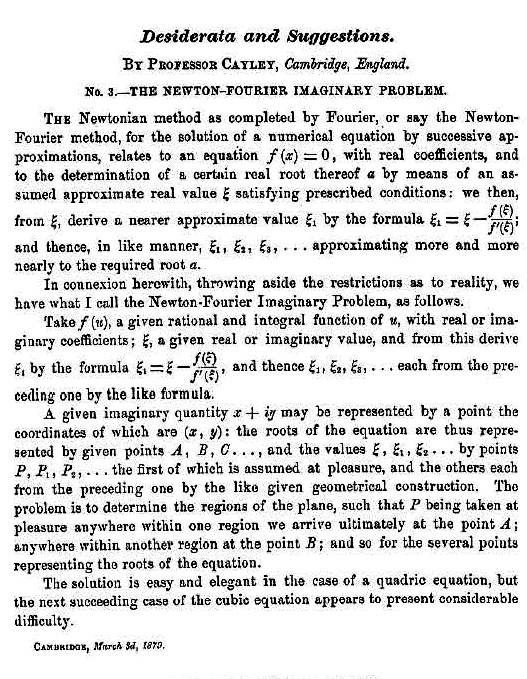
\includegraphics[width=0.45\textwidth]{Cayley1.jpg}
\qquad
 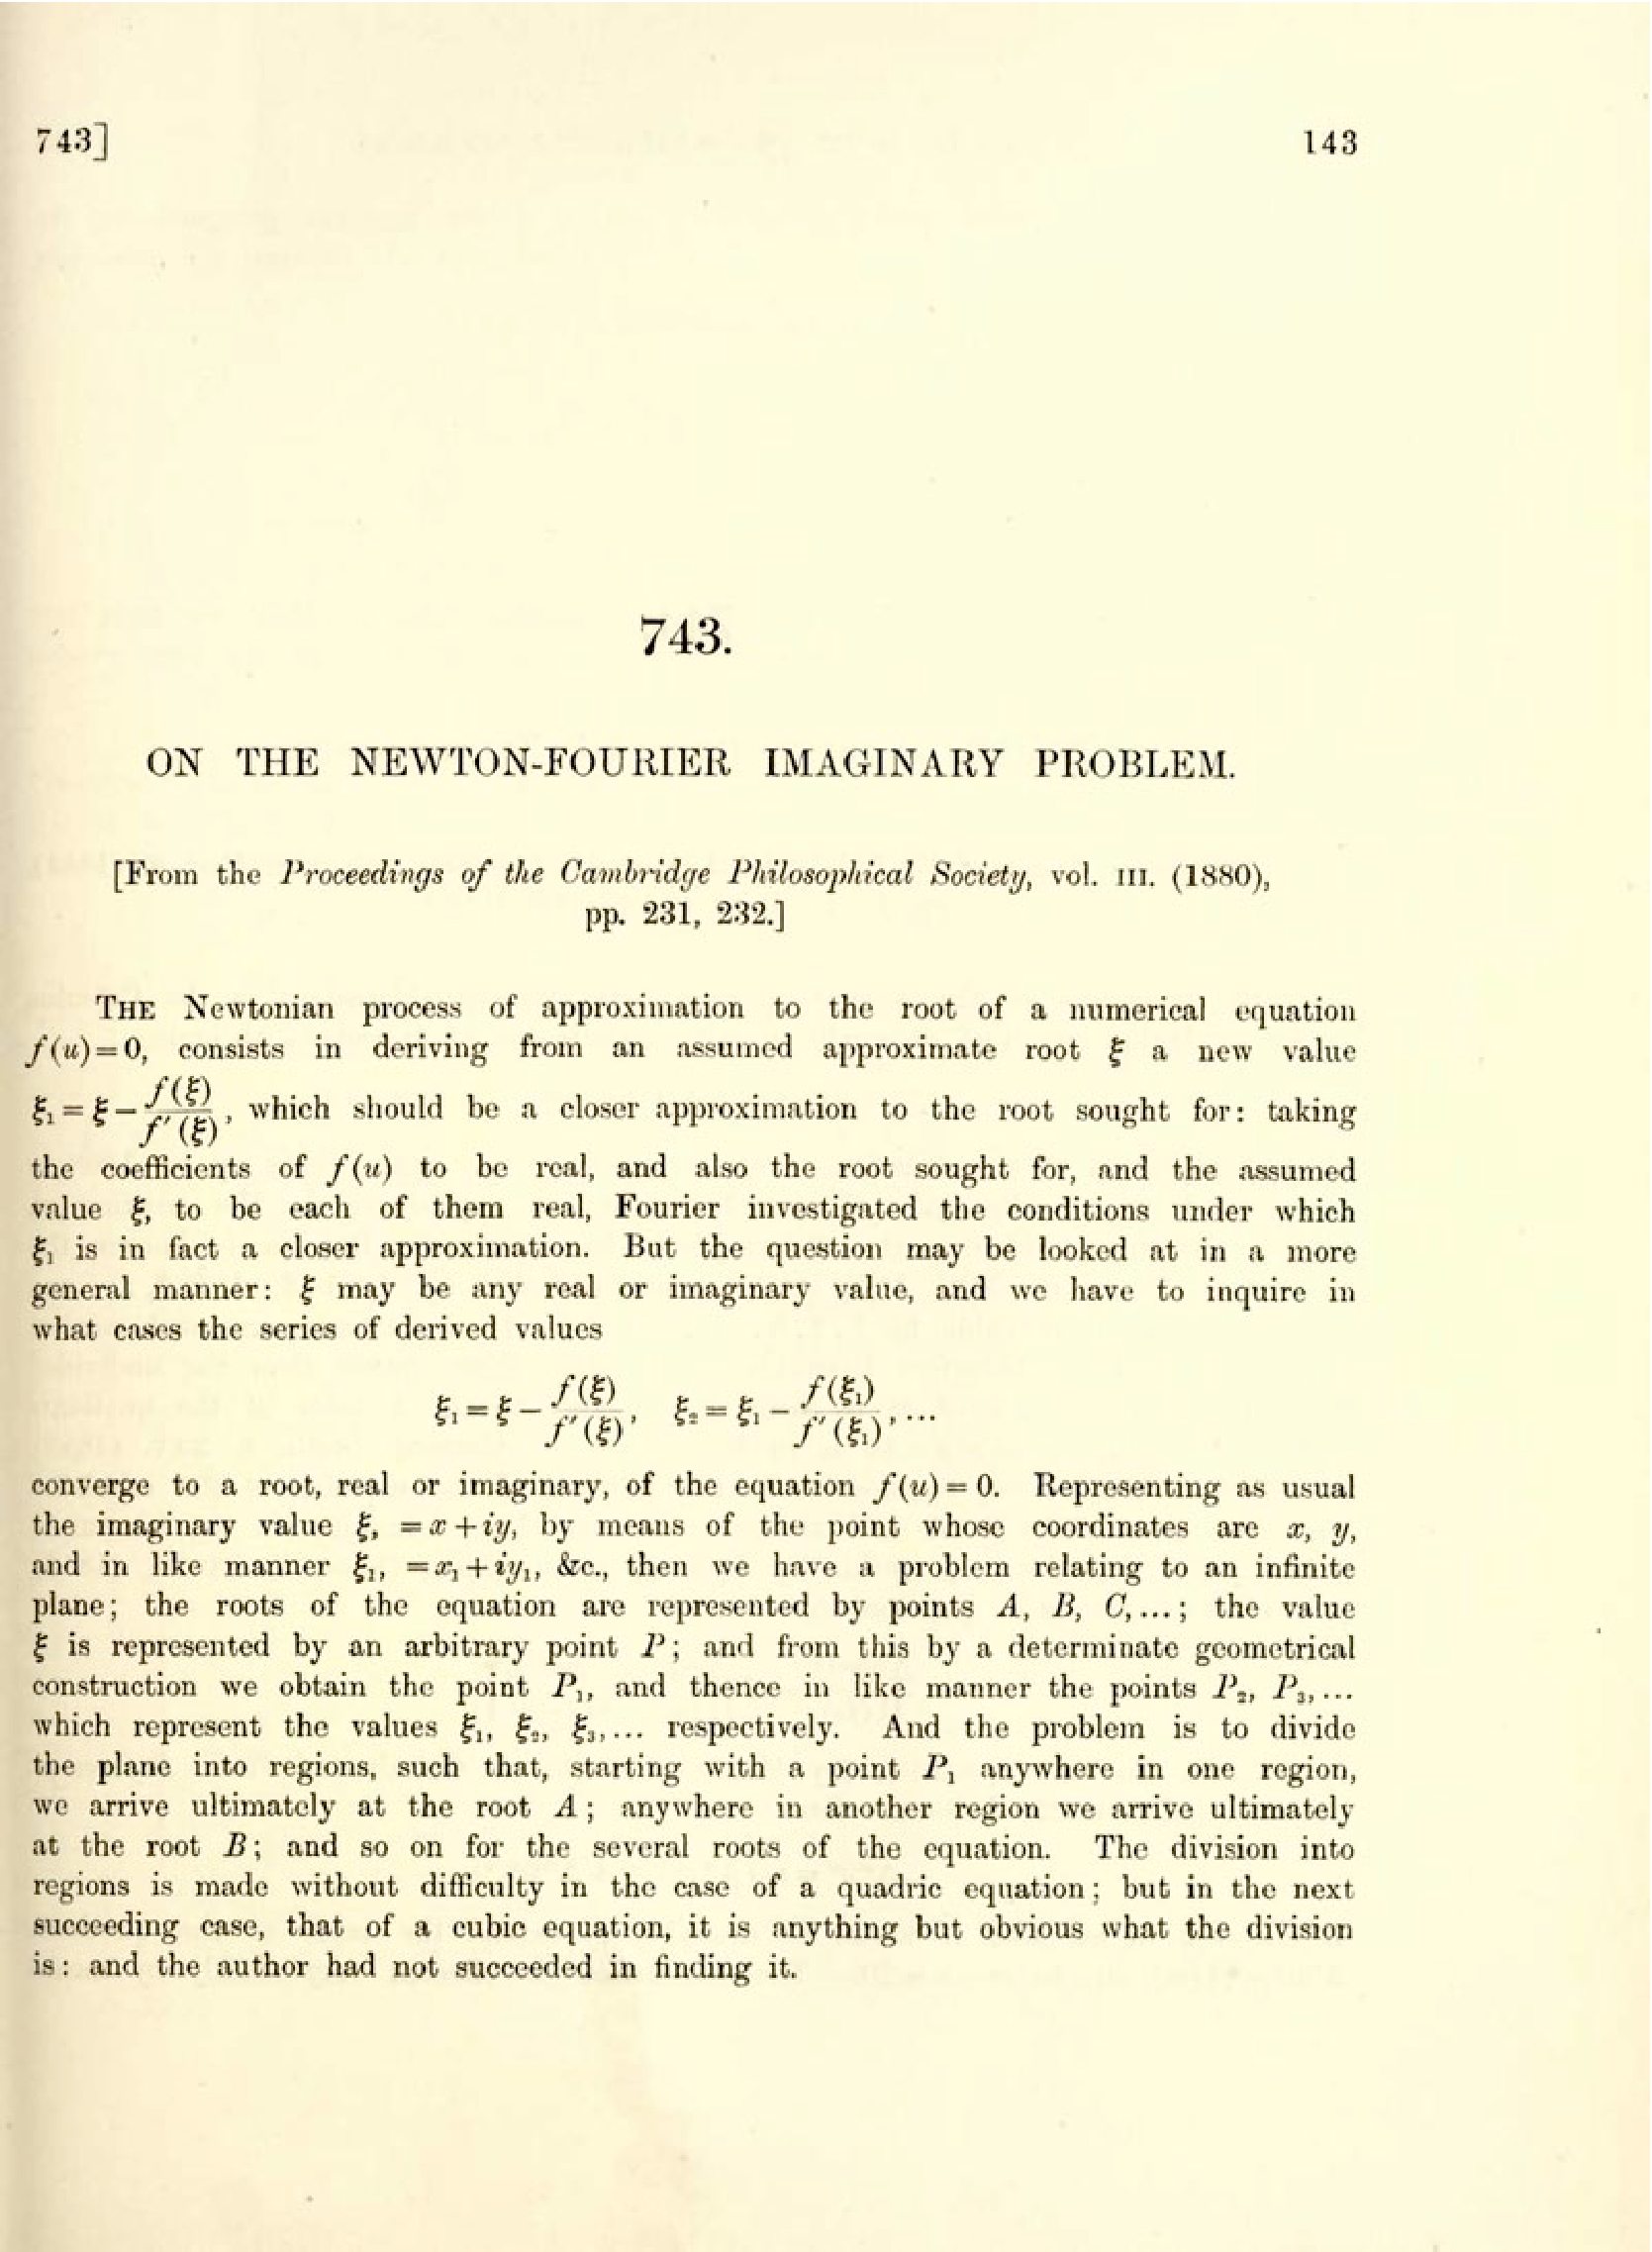
\includegraphics[width=0.45\textwidth]{Cayley2.pdf}
 %\vspace{-1.25cm}
\caption{Los artículos originales de Cayley, de 1879 y 1880 respectivamente,  en los que se pone de manifiesto la dificultad para caracterizar las cuencas de atracción del método de Newton aplicado a polinomios cúbicos.}
 \label{esparam_fig0}
\end{figure}




En la figura~\ref{C4fig:1} mostramos las cuencas de atracción de los polinomios $p(z)=z^2-1$ y $p(z)=z^3-1$. En el primer caso vemos que los puntos de partida situados en el semiplano $\C^-=\{z\in \C: \Re (z)<0 \}$ convergen a la raíz $\z=-1$, mientras que los puntos de partida situados en el semiplano $\C^+=\{z\in \C: \Re (z)>0 \}$ convergen a la raíz $\z=1$. En la separación de ambas regiones, el eje imaginario, en donde el método de Newton presenta un comportamiento caótico. Sin embargo, como vemos en la segunda gráfica de la figura~\ref{C4fig:1}, la situación para el polinomio $p(z)=z^3-1$ es mucho más complicada. La separación entre las cuencas de atracción de las tres raíces, $1$, $(-1+\sqrt{3}i)/2$ y $(-1-\sqrt{3}i)/2$, no es tan diáfana y tiene una estructura mucho más enrevesada.

\begin{figure}[htb]
\centering
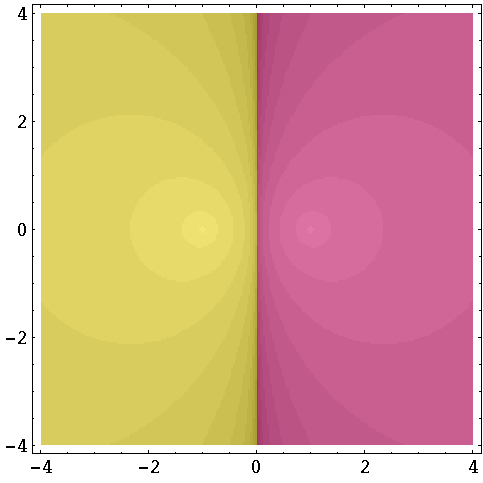
\includegraphics[width=0.45\textwidth]{NDfigura0.pdf}
\qquad
 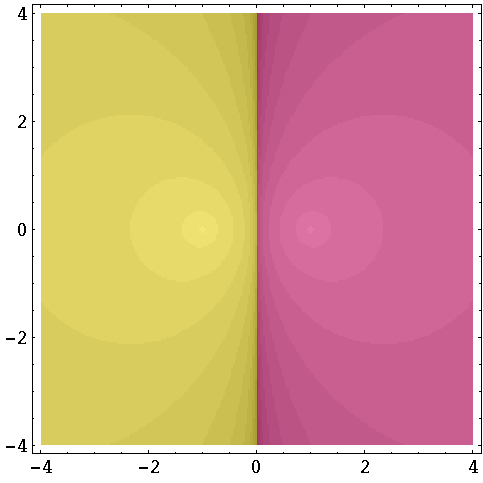
\includegraphics[width=0.45\textwidth]{NDfigura0.pdf}
 %\vspace{-1.25cm}
\caption{A la izquierda se muestran las cuencas de atracción del polinomio $p(z)=z^2-1$ y a la derecha las del polinomio $p(z)=z^3-1$. Las regiones pintadas con el mismo color están formadas por puntos de partida para los cuales el método de Newton converge a la misma raíz del polinomio correspondiente.}
 \label{C4fig:1}
\end{figure}


No es de extrañar, por tanto, que Cayley, que no disponía de los potentes programas de dibujo y cálculo simbólico que tenemos en la actualidad, encontrara dificultades al intentar pasar de una ecuación cuadrática a una cúbica.

Posteriormente, G. Julia y P. Fatou consideran funciones racionales en una forma más general, obteniendo resultados significativos  y sientan el estudio de iteraciones de funciones racionales en el plano complejo extendido, también conocido como la esfera de Riemann. En otras palabras, con sus trabajos comienza en forma sistemática el estudio de los sistemas  dinámicos complejos. La base de sus trabajos fue el estudio realizado por Montel sobre familias normales.%
\index{Fatou, P. J. L.}\index{Julia, G. M.}




\section[Propiedades del método de Newton en $\C$]{Algunas propiedades del método de Newton en el plano complejo} 
\index{Newton, I.!método}

Sea $ p(z) = a_d z^d + \cdots + a_1 z + a_0$, con $ a_d \ne
0$, un polinomio de grado $d $ en $\C$, y sea
$$
N_p(z) = z - \frac{p(z)}{p'(z)} ,
$$
su método de Newton.

Veamos algunas propiedades elementales de la dinámica de
$N_p$:
\begin{itemize}
\item[(1)]  $N_p(z_0) = z_0$ si y sólo si $p(z_0) =  0$,
es decir, los puntos fijos de $ N_p$ son las raíces de~$p$.

\item[(2)]  $ z = \infty$ es siempre un punto fijo de $ N_p$,
y como $   N_p' (\infty) = \frac{d}{d-1}$ este punto fijo es
repulsor. Por lo tanto, si el método de Newton produce un punto
cerca de $ \infty$, sus sucesivas iteraciones se aproximan a
una parte compacta de $\C$.

\item[(3)]  Puesto que $N_p'(z) = \frac{p(z) p''(z)}{(p(z))^2}$,
si $ z_0$ es una raíz simple de $p$,  se tiene que
$ N_p'(z_0) = 0$, esto es, $ z_0$ es un punto fijo
superatractor de $N_p$, lo cual implica que $ N_p$ es
conjugada a la aplicación $ z \to z^k$, para algún $k >
1$ en una vecindad de $z_0$.

\item[(4)]  Las raíces múltiples de $p$ son puntos fijos atractores,
pero no superatractores, de $ N_p $, pues si $z_0$ tiene
mul\-ti\-pli\-ci\-dad $ m > 1$, entonces $ N_p'(z_0) =
\frac{m-1}{m} < 1$.

\item[(5)]  Para polinomios genéricos de grado $ d$, esto es, tienen todas sus raíces distintas, el método
de Newton es una función racional de grado $d$. Cuando el
polinomio tiene raíces múltiples, $N_p$ tiene grado
menor que $d$.

\index{puntos crítico libre}
\item[(6)]  Los puntos críticos de $ N_p$ son las raíces simples
y los puntos de inflexión de $p$. Los puntos críticos
de $N_p$ que no son raíces de $p$ los llamaremos \emph{puntos críticos libres}. 
Recuerde que vimos en la sección
anterior que las propiedades del conjunto de Julia de una
función analítica en $ \overline{\C}$ son
frecuentemente determinadas por las órbitas de sus puntos
críticos.%
\index{Julia, G. M.!conjunto}
 
\item[(7)]  Los puntos críticos de $p$, es decir, las raíces
de $ p'(z) = 0$, son los polos de $N_p$. 
\end{itemize}

Las propiedades  anteriores caracterizan completamente al método de Newton, es decir, tenemos el siguiente resultado.

\begin{teorema}
Una función racional $R:\overline{\C}\longrightarrow \overline{\C}$ de grado $d\ge 2$ es la función de Newton de un polinomio  de grado mayor o igual que $2$ si y sólo si el punto $z=\infty$ es el único punto fijo repulsor y para todos los otros puntos fijos $\xi_1,\ldots, \xi_d\in \C$ existe un número $n_j\in \mathbb{N}$, tal que $R'(\xi_j)=\frac{n_j-1}{n_j}<1$.
\end{teorema}

Este resultado fue probado por G. Saunder en 1984 (\cite{Saunder}). También se le atribuye a J. Head  (\cite{Head}) en 1987 y a K. Nishizawa y M. Fujimura en 1992 (véase \cite{Nishizawa}). En particular, ese resultado contiene el caso del método de Newton para polinomios con raíces simples. Para otros métodos, no se tiene una tal resultado, aún en el caso de polinomios con raíces simples.%
\index{Saunder, G.}\index{Head, J.}\index{Nishizawa, K.}\index{Fujimura, M.}

El primer resultado acerca de la ubicación de los puntos
críticos de un polinomio es el teorema clásico de Gauss-Lucas, que enunciamos a continuación.

\begin{teorema}[Gauss-Lucas, \cite{Lucas}]
\index{teorema de Gauss-Lucas}
Los puntos críticos de un polinomio no contante $p$ están
contenidos en la envoltura convexa de sus  raíces.
\end{teorema}


El siguiente teorema es importante para la descripción global de las posible conducta de los iterados por el método de Newton.


\begin{teorema}[Shishikura, \cite{Shishikura}]
\index{Shishikura, M.}
Sea $R$ un función racional que posee un único punto fijo repulsor o racionalmente indiferente con multiplicador $\lambda=1$, entonces ${\mathcal J}(R)$ es conexo.
\end{teorema}

Como $z=\infty$ es el único punto fijo repulsor para la función de iteración del método de Newton, $N_p$, deducimos la siguiente consecuencia.

\begin{corolario}
\index{Julia, G. M.!conjunto}
Sea $p(z)$ un polinomio complejo, entonces el conjunto de Julia de $N_p$ es conexo.
\end{corolario}

\begin{nota}
Esta propiedad del conjunto de Julia del método de Newton cuando es aplicado a polinomios es una parte fundamental en la demostración del teorema~\ref{HSS} de Hubbard, Schleicher y Sutherland y que en esencia dice que el método de Newton es un algoritmo eficiente para el cálculo de raíces de polinomios. Este teorema, junto con el resultado de Schleicher (véase el teorema~\ref{SchleicherTheo}), nos permite concluir que el método de Newton es, por tantoo, un algoritmo iterativo.%
\index{Hubbard, J. H.}\index{Schleicher, D.}\index{Sutherland, S.}
\end{nota}

\subsection{El método de Newton para polinomios cuadráticos (Con dos raíces)}
$p(z)=(z-a)^m (z-b)^n$
\index{Newton, I.!método}

\index{Cayley, A.!problema}
Como ya se puso de manifiesto al enunciar el problema de Cayley en los antecedentes de este capítulo, el estudio dinámico del método de Newton aplicado a polinomios de la forma $p(z)=(z-a)(z-b)$ es relativamente sencillo. En el teorema~\ref{Cayley-Sch} se vio que $N_p(z)$ es conjugado con la aplicación $g(z)=z^2$. Veamos ahora una nueva demostración de este resultado, poniendo de manifiesto que el conjunto de Julia $J(N_p)$ es la recta que equidista de los puntos $a$ y~$b$.

\begin{teorema}  
\label{Teorema444}
Sea $N_p$ la aplicación de Newton para el polinomio $p(z)=(z-a) (z-b)$, con $a,b\in \C$, $a\ne b$. Entonces $N_p$ es conjugada con la aplicación $z^2$ mediante la transformada de M\"obius $M(z)=(z-a)/(z-b)$. Además $J(N_p)$ es una circunferencia en la esfera compleja que pasa por el punto del infinito, o equivalentemente, $J(N_p)$ es la recta que equidista de los puntos $a$ y $b$ en el plano complejo.
\end{teorema}

\begin{proof}
Se puede comprobar por sustitución directa que $R(z)=M\circ N_p\circ M^{-1}(z)=z^2$, aunque el cálculo puede resultar un poco tedioso. Veamos una demostración alternativa que puede resultar más interesante desde el punto de vista matemático. Lo primero, es observar que
\[
\left.
\begin{array}{ll}
N_p(a)=a  &   M(a)=0   \\
N_p(b)=b  &   M(b)=\infty\\
 N_p(\infty)=\infty  &   M(\infty)=1.
\end{array}
\right.
\]
Entonces, se tiene que:
\[
\left.
\begin{array}{cccccccc}
R: & z & \to & M^{-1}(z) &\to & N_p(M^{-1}(z)) & \to & M(N_p(M^{-1}(z))) \\
 & 0 & \to & a &\to & a & \to & 0 \\
  & \infty & \to & b &\to & b & \to & \infty \\
   & 1 & \to & \infty &\to & \infty & \to & 1.
\end{array}
\right.
\]

$R(z)$ es una aplicación racional de grado 2 (como $N_p(z)$) que fija el 0, el $\infty$ y el 1. Además,
$$
R'(z)=M'(N_p(M^{-1}(z))) N_p'(M^{-1}(z)) (M^{-1})'(z)
$$
$$
=
\frac{M'(N_p(M^{-1}(z))) N_p'(M^{-1}(z))}{M'(M^{-1}(z))}.
$$
Como $M'(z)=(a-b)/(z-b)^2$ y $N_p'(z)=L_p(z)=p(z)p''(z)/p'(z)^2$, se tiene que
$$
R'(0)=
\frac{M'(N_p(a)) N_p'(a)}{M'(a)}=N_p'(a)=0 \quad (M'(a)\ne 0).
$$
Por otra parte, como $M'(b)=\infty$,
$$
R'(\infty)=
\lim_{x\to b}\frac{M'(N_p(x)) N_p'(x)}{M'(x)}=\lim_{x\to b}\frac{(x-b)^2}{(N_p(x)-b)^2} N_p'(x)= \lim_{x\to b}\frac{1}{N_p'(x)} =\infty.
$$
Así, $R(z)$ tiene una raíz doble en $z=0$, luego es de la forma
$$
R(z)=\frac{z^2}{\alpha z^2+\beta z+\gamma}.
$$
Como $R(\infty)=\infty$, $\alpha=0$. Como $R'(\infty)=\infty$ y
$$
R'(\infty)=\lim_{z\to \infty}\frac{2z(\beta z+\gamma)-\beta z^2}{(\beta z+\gamma)^2}=\frac{1}{\beta},
$$
se sigue que $\beta=0$. Por último, como $R(1)=1$, $\gamma=1$ y $R(z)=z^2$.
\end{proof}



\subsection{El método de Newton para polinomios cúbicos con raíces múltiples} 
\index{Newton, I.!método}

Una ligera variante del estudio realizado en la sección anterior nos permite obtener algunas conclusiones acerca del comportamiento del método de Newton cuando aparecen raíces múltiples.
Lo primero observación general que podemos hacer es que cuando se aplica el método de Newton a un polinomio de grado $d$, la función de iteración resultante tiene grado $d$ cuando las raíces son simples. Sin embargo, cuando las raíces son múltiples, el grado de la función de iteración es menor estrictamente que $d$.
Consideramos en esta sección el caso del polinomio
\begin{equation}\label{eq5}
p(z)=(z-a)^2(z-b).
\end{equation}
 En este caso, particularmente sencillo, el polinomio tiene una raíz doble y una raíz simple. Analizaremos las dinámicas del método de Newton y  estudiaremos cómo son las cuencas de atracción de las raíces de $p$. Veremos que el comportamiento es totalmente distinto a cuando las raíces del polinomio son simples.

\begin{figure}[htb]
\centering
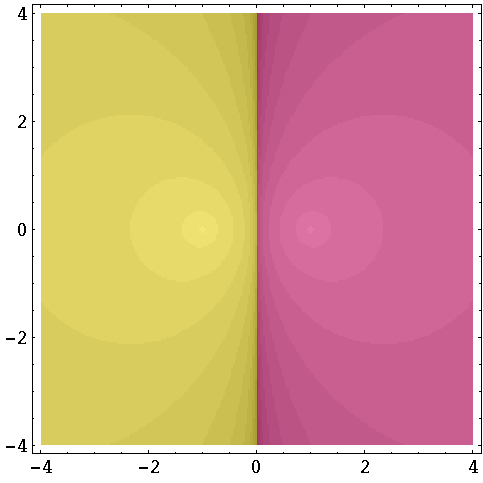
\includegraphics[width=0.5\textwidth]{NDfigura0.pdf}
\caption{Cuencas de atracción de las raíces, $z=-1$ y  $z=1$ para el método de Newton aplicado al polinomio $p(z)=(z-1)^2(z+1)$.}
\label{fig4:41}
\end{figure}

 En primer lugar, mediante cambios de variable afines, el estudio del método de Newton aplicado a polinomios de la forma (\ref{eq5}), puede reducirse al estudio del polinomio $p(z)=(z-1)^2(z+1)$. En este caso, la función de iteración del método de Newton es de la forma
 $$
 N_p(z)=\frac{2z^2+z+1}{1+3z}.
 $$
 Esta función tiene un punto fijo superatractor en $z=-1$ y un punto fijo atractor en $z=1$, con multiplicador asociado $1/2$. Además, el punto del infinito es un punto fijo repulsor con multiplicador asociado $3/2$. En la figura~\ref{fig4:41} se muestran las cuencas de atracción de las dos raíces, $z=-1$ y  $z=1$. Como se puede apreciar en la figura, la cuenca de atracción de la raíz múltiple, en este caso, $z=1$, <<invade>> la cuenca de atracción de la otra raíz, $z=-1$.  En este caso, la presencia  de dos raíces, una múltiple y otra simple,  hace que se pierda la simetría a la que hace referencia el teorema~\ref{Teorema444}.

Por otra parte, para el caso de polinomios con raíces múltiples de la forma (\ref{eq5}) la iteración de Newton, $N_p(z)$, es conjugada mediante la transformada de M\"obius $M(z)=(z-a)/(z-b)$ con la aplicación $z(z+1)/2$ definida en el plano complejo ampliado $\hat \C$. El correspondiente conjunto de Julia  se muestra en la figura~\ref{figura1230}.
\begin{figure}[htbp]
    \centering
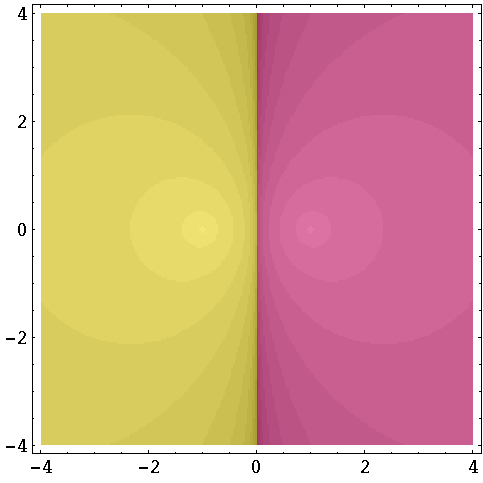
\includegraphics[width=0.45\textwidth]{NDfigura0.pdf}
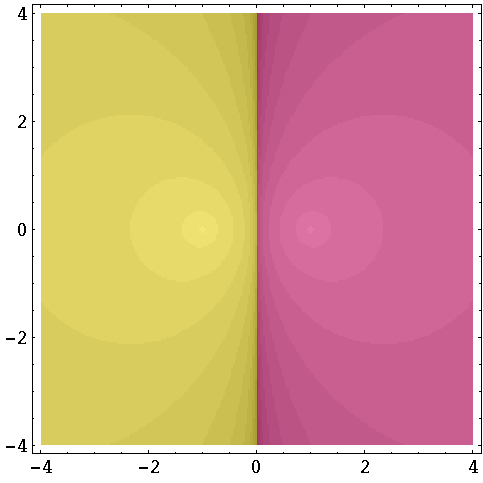
\includegraphics[width=0.45\textwidth]{NDfigura0.pdf}
    \caption{Cuencas de atraccción asociadas a las funciones de iteración  $z(z+1)/2$ y $z^2-3/4$, relacionadas respectivamente con el método de Newton y el método de Newton para raíces múltiples.}
    \label{figura1230}
 \end{figure}
 
Si se conoce la multiplicidad $m$ de la raíz a aproximar,  el conocido como método de Newton para raíces múltiples,
\begin{equation}\label{NwMul}
N_m(z)=z-m\frac{p(z)}{p'(z)}
\end{equation}
tiene la ventaja de que recupera el orden de convergencia cuadrático al aproximar la raíz múltiple. El estudio de la dinámica del método~(\ref{NwMul})
para  polinomios de la forma (\ref{eq5}) lo realizó Gilbert \cite{Gilbert}. En ese trabajo, se prueba que la correspondiente función de iteración para polinomios de la forma (\ref{eq5}) es
\begin{equation}\label{NwMul7}
N_2(z)=z-2\frac{p(z)}{p'(z)}=\frac{z^2+az-2ab}{3z-a-2b}.
\end{equation}
Esta función racional  es conjugada con la aplicación $z^2-3/4$ mediante la transformada de M\"obius 
$$
M(z)=\frac{3z+a-4b}{2(z-a)}.
$$ 
El comportamiento dinámico de la función polinómica $z^2-3/4$ es bien conocido (véase \cite{Beardon}, por ejemplo). En el segundo gráfico de la figura~\ref{figura1230} se muestra el conjunto de Julia  para $z^2-3/4$, que es la frontera de la región de negro. Nótese que en este caso, las raíces $a$ y $b$ del polinomio (\ref{eq5}) se transforman por $M$ en los puntos
$$
M(a)=\infty, \quad M(b)=-\frac{1}{2}.
$$
Estos dos puntos $\infty$ y $-1/2$, junto con el punto $3/2$, son los puntos fijos del polinomio $z^2-3/4$. $\infty$ es un punto fijo superatractor, $-1/2$ es un punto fijo indiferente y $3/2$ es un punto fijo repulsor. Deshaciendo los cambios se concluye que el método de Newton para raíces múltiples (\ref{NwMul7}) ha transformado la raíz múltiple $a$ en un punto fijo superatractor. Como contrapartida, la otra raíz, $b$, pasa a ser un punto fijo indiferente. Por último $\infty$ es un punto fijo repulsor para~(\ref{NwMul7}).

El segundo gráfico de la figura~\ref{figura1230}  muestra la cuenca de atracción de $\infty$ como punto fijo de $z^2-3/4$. Los puntos de la región de negro convergen al punto fijo indiferente $-1/2$, aunque, en este caso la convergencia es extremadamente lenta.

Otra variante del método de Newton para ecuaciones con raíces múltiples viene dada por
\begin{equation}\label{NwMul2}
\hat{N}_p(z)=z-\frac{1}{1-L_p(z)}\frac{p(z)}{p'(z)}, \quad L_p(z)=\frac{p(z)p''(z)}{p'(z)^2}.
\end{equation}
$\hat{N}_p(z)$ se obtiene aplicando el método de Newton a la función racional $p(z)/p'(z)$. Para polinomios de la forma (\ref{eq5}), el método~\ref{NwMul2}
 es conjugado con la aplicación $-z^2$ mediante la transformada de Möbius $M(z)=(z-a)/(z-b)$. Por lo tanto, su conjunto de Julia  es la circunferencia unidad y sus dinámicas son similares al método de Newton para raíces simples (véase el teorema~\ref{Teorema444}).



\subsection{El método de Newton para polinomios cúbicos}
\index{Newton, I.!método}

Sea $p(z)= a_3z^3+a_2z^2+a_1z+a_0$  un polinomio cúbico con
sus tres raíces  $a$, $b$ y $c$ distintas, las
cuales suponemos ordenadas por sus módulos, es decir,  $0 \le
|a| \le |b| \le |c|$.

Pongamos $ T^{-1}(z) = \alpha z + \beta $, y encontremos los
coeficientes $ \alpha$ y $ \beta$  de modo que $
T^{-1}(a) = 0$ y $ T^{-1}(c) = 1$. Tenemos entonces que $
\alpha = \frac{1}{c-a}$ y $ \beta = - \frac{a}{c-a}$, por lo
tanto, $ T^{-1}(z) = \frac{z}{c-a} - \frac{a}{c-a}$, y en
consecuencia $ T(z) = (c-a) z + a$. Aplicando esta
transformación $T$ en el teorema de  reescalamiento\index{reescalamiento}
anterior (teorema~\ref{reescalamiento}), obtenemos
$$
q(z) = p \circ T (z)  = p ( (c-a) z + a)= (c-a)^3 z \left( z -
\frac{b-a}{c-a}\right) ( z -1 ) .
$$
Haciendo, $ \lambda = ( c - a)^3$ y $ \rho =
(b-a)/(c-a)$, obtenemos
$$
q(z) = \lambda^3  z ( z - 1)( z - \rho ) .
$$

Por otra parte, es fácil ver que si $ f(z) = \alpha g(z)$,
entonces  $ N_f(z) =
N_g(z)$.

En consecuencia,  haciendo 
\begin{equation}\label{prho}
p_{\rho}(z) = z (z-1)(z-\rho)
\end{equation}
 y
denotando por $N_{\rho}$ a su correspondiente función de iteración para el método de Newton,
\begin{equation}\label{Nro}
 N_{\rho}(z)=z-\frac{ z (z-1)(z-\rho)}{3 z^2-2 \rho z-2 z+\rho},
\end{equation}
 tenemos
probado el siguiente resultado, que establece que para conocer la
di\-ná\-mi\-ca de la método de Newton de un polinomio
cúbico debemos conocer la dinámica de la función racional $N_{\rho}$, donde $ \rho \in \C$ es un parámetro.

\begin{teorema}
Sea $ p(z)$ un polinomio cúbico con sus tres raíces
distintas. Entonces, $ N_p$ es conjugado topológicamente con
$N_{\rho}$ definida en~(\ref{Nro}).
\end{teorema}

Notemos que el caso $ \rho = 0 $ se reduce al estudio del método de Newton aplicado al polinomio $ p_0 (z) = z^2 (z-1) = z^3 -
z^2$. Este polinomio tiene en $0$ una raíz doble y su comportamiento dinámico es similar al del polinomio que aparece en la figura~\ref{fig4:41}.

En este caso, tenemos
$$
N_{\rho} (z) =  z -
 \frac{z^3 - (\rho + 1) z^2 + \rho z}{ 3 z^2 - 2 (\rho + 1 )z + \rho}
= \frac{2 z^3 - (\rho + 1 ) z^2}{ 3 z^2 - 2 (\rho + 1) z + \rho}
$$
y
$$
N_{\rho}'(z) = \frac{( z^3 - (\rho +1 )z^2 + \rho z) ( 6 z - 2
(\rho +1)}{ (3 z^2 - 2 (\rho + 1) z + \rho )^2}.
$$
Un estudio sobre de familia fue hecho por Curry, Garnett  y
Sullivan  \cite{CGS}.


En este caso,  $ N_{\rho}'(z) = 0 $ si y sólo si $p_{\rho}
(z) = 0$  o $ p_{\rho}''(z) =
0$.  En consecuencia, el conjunto de puntos críticos de $ N_{\rho}$ está formado por  las tres raíces de $ p_{\rho}$ junto con el punto $ z = \frac{\rho +1 }{3}$. Los puntos
críticos de $N_{\rho}$ que no son raíces de $
p_{\rho}$ se llaman \emph{puntos críticos libres}.%
\index{punto crítico libre}

El estudio de las órbitas de los puntos críticos libres da mucha información sobre el comportamiento dinámico de un método. En concreto, para determinar si
existen órbitas periódicas atractoras para $N_{\rho}$,
distintas de las raíces de $ p_{\rho}$, debemos responder
a la pregunta siguiente: ¿para  qué valores de $\rho$, la órbita del punto crítico libre, 
$$
N_{\rho}^{n}\left(\frac{\rho+1}{3}\right)
$$ 
es una órbita periódica
atractora?



En la pregunta anterior debemos excluir los casos
 $ \rho = -1$, $ \rho = 2 $ y
$ \rho = 1/2$ para los cuales el punto fijo extraño coincide con alguna de las raíces del polinomio   $ p_{\rho}$.


Una manera de responder a la pregunta anterior es colorear el espacio de parámetros $\rho\in\C$ de acuerdo a la convergencia del punto crítico libre $(\rho+1)/3$, tal y como se hace en la figura~\ref{esparam_fig0}. Si la órbita de $(\rho+1)/3$ converge a 0, 1 o $\rho$, el valor del correspondiente parámetro $\rho$ se colorea en amarillo, cian o magenta respectivamente.

\begin{figure}[htb]
\centering
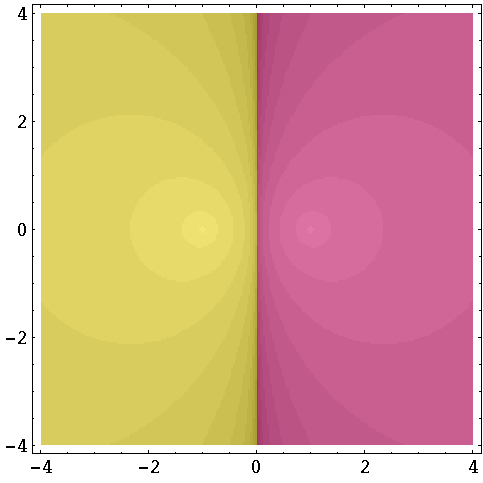
\includegraphics[width=0.45\textwidth]{NDfigura0.pdf}
\qquad
 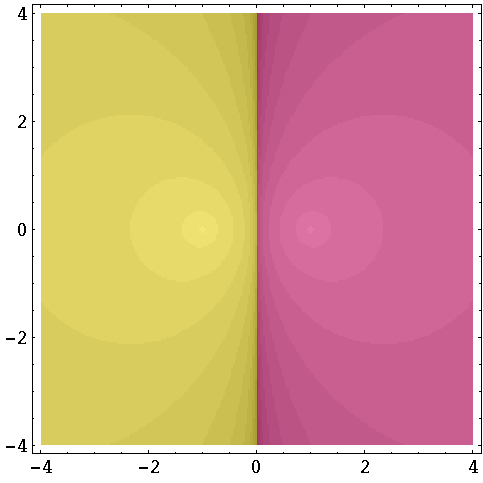
\includegraphics[width=0.45\textwidth]{NDfigura0.pdf}
 %\vspace{-1.25cm}
\caption{Representación gráfica del espacio de parámetros asociado a la función de iteración $N_{\rho}(z)$ definida en~(\ref{Nro}) y asociada a los polinomios de la forma $p_{\rho}(z) = z (z-1)(z-\rho)$. La figura de la derecha muestra una ampliación de una zona negra en la que se aprecia  un conjunto de tipo Mandelbrot.}
 \label{esparam_fig0}
\end{figure}


Como se aprecia en la figura~\ref{esparam_fig0}, existen regiones abiertas en el \emph{espacio de parámetros} tales que, si $\rho$ pertenece a estas regiones entonces existen regiones abiertas en el plano complejo de forma que 
$N_{\rho}(z)$ definida en~(\ref{Nro}) no converge a ninguna de las raíces del polinomio $p_{\rho}(z)$ definido en~(\ref{prho}). Las regiones coloreadas en negro en el espacio de parámetros están formadas por los valores de $\rho$ para los cuales la sucesión
$$
N_{\rho}^{n}\left(\frac{\rho+1}{3}\right)
$$ 
va a parar a  un ciclo atractor.

La parametrización de los polinomios cúbicos considerada en (\ref{prho}) no es la única. Otra parametrización muy habitual (véase \cite{Roberts}) es la siguiente:
\begin{equation}\label{pnu}
p_{\mu}(z)=(z^2-1)(z-\mu), \quad \mu\in\C.
\end{equation}
La correspondiente función de iteración para el método de Newton es
\begin{equation}\label{Nnu}
 N_{\mu}(z)=\frac{ 2z^3-\mu z^2-\mu}{3 z^2-2 \mu z-1}.
\end{equation}

En este caso, el punto crítico libre asociado al método de Newton es la única raíz de $p''_{\mu}(z)=0$, es decir, $z=\mu/3$. Podemos realizar una reflexiones similares al caso anterior y colorear el espacio de parámetros conforme a la convergencia del punto crítico libre, amarillo, cian o magenta si la órbita de $\mu/3$ converge a 
$\mu$, 1 o $-1$ respectivamente, tal y como se muestra en la figura~\ref{esparam_fig1}.  De nuevo, las regiones coloreadas en negro en el espacio de parámetros están formadas por los valores de $\mu$ para los cuales la sucesión
$$
N_{\mu}^{n}\left(\frac{\mu}{3}\right)
$$ 
va a parar a  un ciclo atractor.

\begin{figure}[htb]
\centering
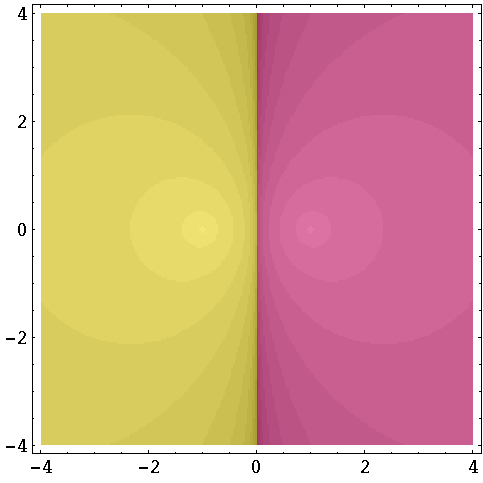
\includegraphics[width=0.45\textwidth]{NDfigura0.pdf}
\qquad
 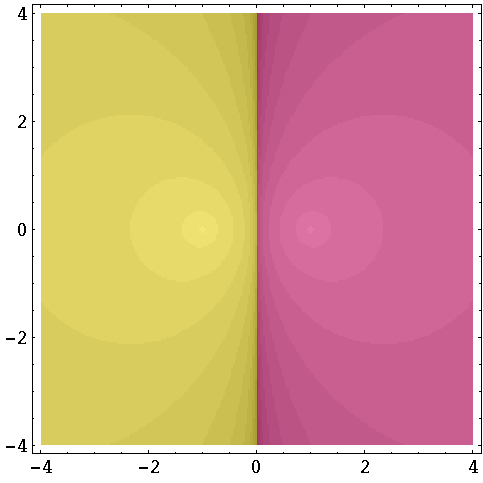
\includegraphics[width=0.45\textwidth]{NDfigura0.pdf}
 %\vspace{-1.25cm}
\caption{Representación gráfica del espacio de parámetros asociado a la función de iteración del método de Newton para los polinomios~(\ref{pnu}). La figura de la derecha muestra una ampliación de una zona negra en la que se aprecia un conjunto de tipo Mandelbrot similar al de la figura~\ref{esparam_fig0}.}\index{Mandelbrot, B.!conjunto}
\label{esparam_fig1}
\end{figure}




Por último, consideramos  otra parametrización muy conocida (véase \cite{PlazaRomero}), como es la siguiente:
\begin{equation}\label{plambda}
p_{\lambda}(z)=z^3+(\lambda-1)z-\lambda, \quad \lambda\in\C.
\end{equation}
Denotamos $N_{\lambda}(z)$ a la función de iteración del método de Newton aplicado a los polinomios de la forma~(\ref{plambda}):
\begin{equation}\label{Nlambda}
N_{\lambda}(z)=\frac{2z^3+\lambda}{3z^2+\lambda-1}.
\end{equation}
\index{espacio de parámetros}%
En este caso, el punto crítico libre asociado al método de Newton es la única raíz de $p''_{\lambda}(z)=0$, es decir, $z=0$. 

Las regiones coloreadas en negro en el espacio de parámetros de la  figura~\ref{esparam_fig2} están formadas por los valores de $\lambda$ para los cuales la sucesión
$$
N_{\lambda}^{n}(0)
$$ 
va a parar a  un ciclo atractor.

\begin{figure}[htb]
\centering
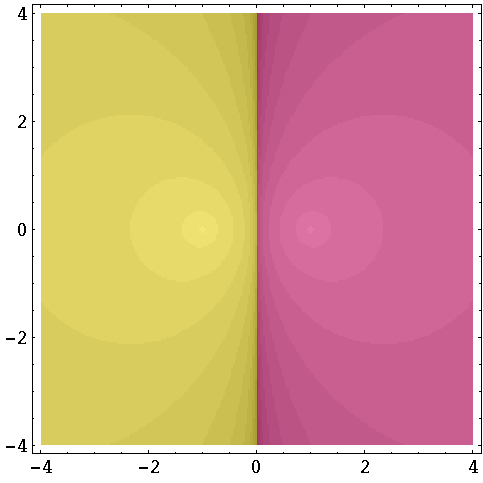
\includegraphics[width=0.45\textwidth]{NDfigura0.pdf}
\qquad
 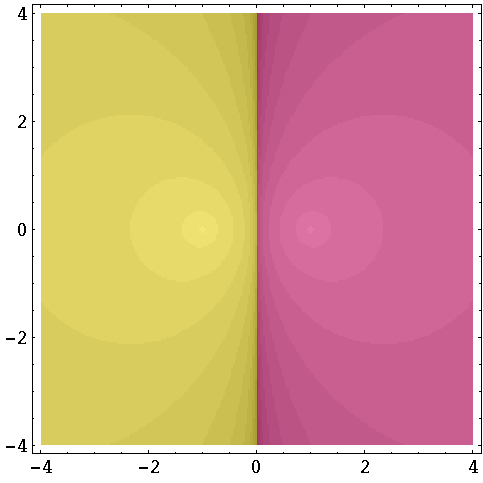
\includegraphics[width=0.45\textwidth]{NDfigura0.pdf}
 %\vspace{-1.25cm}
\caption{Representación gráfica del espacio de parámetros asociado a la función de iteración $N_{\lambda}(z)$ definida en~(\ref{Nlambda}) y la correspondiente ampliación mostrando un conjunto de tipo Mandelbrot.}\index{Mandelbrot, B.!conjunto}
 \label{esparam_fig2}
\end{figure}


La figura~\ref{esparam_fig3} muestra las cuencas de atracción del método de Newton para un polinomio $p_{\lambda}(z)$ definido en~(\ref{plambda}) y tomando $\lambda$ en una de las zonas negras del espacio de parámetros. Como vemos aparecen <<agujeros negros>> originados por la presencia de ciclos atractores. En concreto, en este caso se tiene que la órbita del punto crítico libre $z=0$ es atraída por el 3-ciclo
$$
\{1.02169 - 1.04136i, 0.620968  - 0.632698 i, -0.00204529 + 
 0.00527748 i \}.
$$

\begin{figure}[htb]
\centering
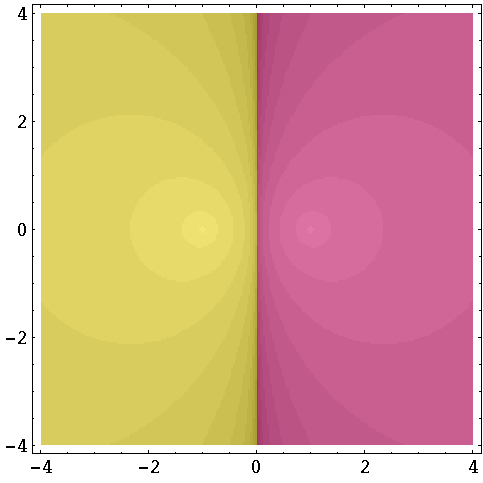
\includegraphics[width=0.45\textwidth]{NDfigura0.pdf}
\qquad
 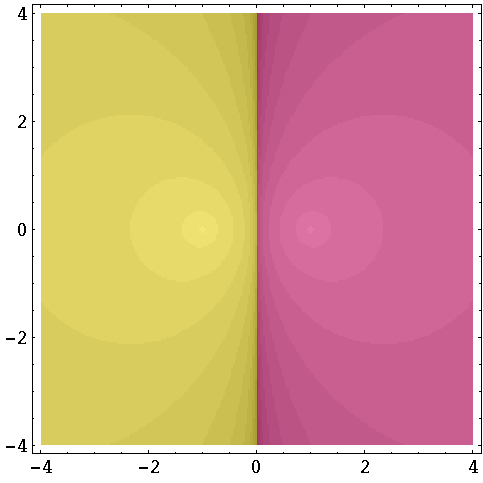
\includegraphics[width=0.45\textwidth]{NDfigura0.pdf}
 %\vspace{-1.25cm}
\caption{Cuencas de atracción del método de Newton aplicado al  polinomio $p_{\lambda}(z)=z^3+(\lambda-1)z-\lambda$ con $\lambda=1.02+0.96i$ y una ampliación de la zona negra que se genera entorno al punto crítico libre $z=0$.}
 \label{esparam_fig3}
\end{figure}


\subsection{El método de Newton para polinomios de grados 4 y 5} 
\index{Newton, I.!método}

Como hemos visto en el apartado anterior, el estudio dinámico del método de Newton aplicado a polinomios de tercer grado se reduce al estudio de una función racional dependiente de un parámetro, en concreto~(\ref{Nro}). Evidentemente, al aumentar el grado de los polinomios también lo hará el número de parámetros involucrados en la correspondiente función racional asociada al método de Newton.

No obstante, existen algunas manipulaciones algebraicas que permiten reducir el número de coeficientes que aparecen en una ecuación polinómica. En concreto, la conocida como \emph{transformación de Tschirnhaus} (\cite{Dickson}) permite transformar la ecuación\index{transformación de Tschirnhaus}
$$
z^n+a_{n-1}z^{n-1}+\cdots+a_{1}z+a_0=0, \quad n>2,
$$
en otra ecuación polinómica donde no aparecen los términos en $z^{n-1}$ y $z^{n-2}$, es decir,
$$
z^n+b_{n-3}z^{n-3}+\cdots+b_{1}z+b_0=0, \quad n>2.
$$
El resultado original de Tschirnhaus apareció publicado en \emph{Acta Eruditorum} en 1683. Más adelante, en 1786, E. S. Bring probó que una ecuación polinómica de grado 5 puede reducirse a una del tipo
$$
z^5+az+b=0.
$$
Finalmente, en 1834 G. B. Jerrard demostró que en ecuaciones polinómicas de grado mayor que 3 se puede encontrar  una transformación de Tschirnhaus en la que no aparecen los términos en $z^{n-1}$, $z^{n-2}$ y $z^{n-3}$, es decir, del tipo
$$
z^n+c_{n-4}z^{n-4}+\cdots+c_{1}z+c_0=0, \quad n>3.
$$

Estas transformaciones se basan en complicadas manipulaciones algebraicas sobre las raíces de la ecuación (véase \cite{WeissBJ}). Estas manipulaciones no conservan las propiedades dinámicas. En efecto, como se vio en el ejemplo~(\ref{ejem4.5}), el  método de Newton aplicado al polinomio $z^3-2z+2$ tiene un 2-ciclo atractor de la forma $\{0,1\}$. Dicho polinomio puede ser transformado en uno de la forma $p(z)=z^3-\lambda^3$, $\lambda\in \C$, por la correspondiente transformación de Tschirnhaus. A su vez, el método de Newton aplicado al polinomio anterior,
$$
N_p(z)=z-\frac{z^3-\lambda^3}{3z^2}=\frac{2z^3+\lambda^3}{3z^2}
$$
 es conjugado topológicamente, mediante la aplicación afín $h(z)=z/\lambda$, con el método de Newton aplicado al polinomio $q(z)=z^3-1$,
$$
N_q(z)=z-\frac{z^3-1}{3z^2}=\frac{2z^3+1}{3z^2}.
$$
En efecto,
$$
h\circ N_p(z)=\frac{2z^3+\lambda^3}{3\lambda z^2}=N_q\circ h(z).
$$
Pero como se aprecia en las figuras~\ref{C4fig:1} y~\ref{fig44:2}, el comportamiento dinámico del método de Newton aplicado a los polinomios $q(z)=z^3-1$ y $z^3-2z+2$ es muy diferente. De hecho, en el primer caso no aparecen $n$-ciclos atractores con $n\ge 2$, luego su dinámica no puede ser equivalente a la del método de Newton aplicado al polinomio $z^3-2z+2$, que sí presenta un 2-ciclo atractor.

Para ver que $N_p(z)$ no tiene 2-ciclos atractores, calculamos los puntos fijos de 
$$
N_p^2(z)=\frac{16 z^9+51 z^6+12z^3+2}{9 z^2 \left(2  z^3+1\right)^2}.
$$
Tenemos que $N_p^2(z)=z$ si y sólo si $z^3=1$ o $20 z^6+5 z^3+2=0$. Los 2-ciclos aparecen entre las raíces $\xi_j$, $j=1,\dots, 6$ de la segunda ecuación. Pero en todas ellas se cumple que 
$$
|N'_p(\xi_j)|\approx 2.45>1,
$$
luego ningún 2-ciclo es atractor.

Las expresiones simplificadas de polinomios de cuarto y quinto grado que aparecen después de aplicar las transformaciones de Tschirnhaus o de Bring-Jerrard, motivan el estudio del método de Newton para ecuaciones de la forma $z^4+az+b^4=0$ o $z^5+az+b^5=0$ como casos particulares de ecuaciones polinómicas de cuarto y quinto grado respectivamente. En concreto, para la ecuación de quinto grado anterior puede verse un estudio detallado de la dinámica del método de Newton en~\cite{Balibrea}.










